documentclass[]
\usepackage{tikz}
\usetikzlibrary{decorations.pathmorphing}

\begin{document}

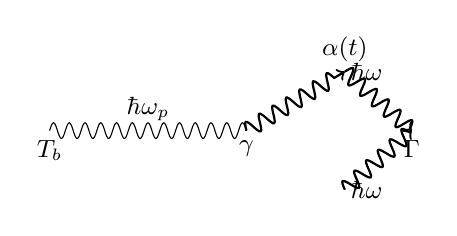
\begin{tikzpicture}[font=\small]
\draw[decorate,decoration={coil,amplitude=1mm,segment length=2mm,aspect=0}]
(-3.75,0)--node[midway,above,sloped]{$\hbar \omega_p$}(-1.25,0);
\draw[->,decorate,decoration={coil,amplitude=1mm,segment length=2mm,aspect=0},thick]
(-1.25,0)--(0,.75);
\draw[->,decorate,decoration={coil,amplitude=1mm,segment length=2mm,aspect=0},thick]
(0,-.75)--(.85,0);
\draw[->,decorate,decoration={coil,amplitude=1mm,segment length=2mm,aspect=0},thick]
(0,.75)--(.85,0);
\node at (.6,.75)[left]{$\hbar \omega$};
\node at (.6,-.75)[left]{$\hbar \omega$};
\node at (-1.25,0)[below]{\small{$\gamma$}};
\node at (0,.75)[above]{\small{$\alpha(t)$}};
\node at (.85,0)[below]{\small{$\Gamma$}};
\node at (-3.75,0)[below]{\small{$T_b$}};
\end{tikzpicture}

\end{document}